\begin{anexosenv}

    \partanexos
    \chapter{Documento de Arquitetura}
    \label{adoarquitetura}
    \section{Introdução}
    Este documento descreve a arquitetura e tecnologias da solução de \textit{software}, utilizadas no desenvolvido do sistema de auxílio na detecção da doença de Parkinson avaliando o Tremor em Repouso. Desenvolvido pelos alunos de Trabalho de Conclusão de Curso 2 da Universidade de Brasília.

    Essa solução de \textit{software} trata-se de uma aplicação \textit{web}, na qual pode-se facilmente ser migrada para uma aplicação \textit{mobile} em projetos futuros.

    \section{Tecnologias}
    \subsection{SPA}
    SPA (sigla do inglês: \textit{Single Page Application}, Aplicativo de página única), consiste em uma aplicação \textit{web} em uma única página, fornecendo uma experiência de usuário semelhante a um aplicativo Desktop, sem recarregamentos da página.

   O SPA foi adotado devido a sua vantagem de performance no consumo de dados e na experiência do usuário.

    \subsection{REST}
    Baseado no protocolo de comunicação de rede HTTP, sendo simples, rápida e com uma fácil comunicação entre clientes e servidores. Funciona com objetos em formato JSON, e os métodos definidos no protocolo HTTP ( POST, GET, PUT e DELETE) possibilitando assim uma eficiente e rápida troca de informação.

   Foi adotado devido a seu leve consumo de dados, além de possuir uma fácil implementação.

    \section{Representação da Arquitetura}
    A arquitetura se baseia em dois modelos arquiteturais, REST e SPA, interligados com um modelo de aprendizado de máquinas. No caso a \textit{Random Forest} ou o SVM, como observado na Figura \ref{diagramadepacotes}. Deste modo a aplicação possui três pacotes:

    \begin{itemize}
        \item \textit{Machine Learning models};
        \item API;
        \item \textit{web}.
    \end{itemize}


   \section{Visão Lógica}
   \subsection{Diagrama de Pacotes}
   \begin{figure}[!htb]
        \centering
        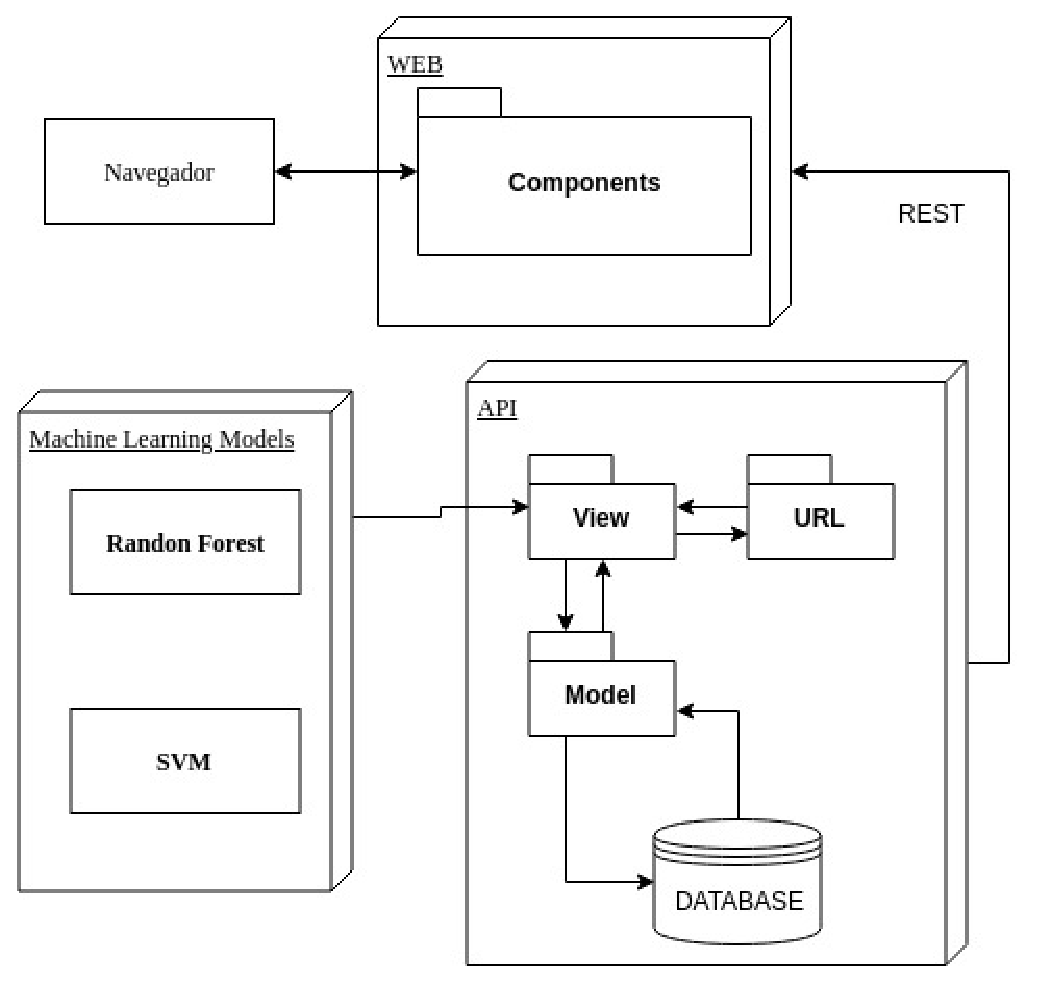
\includegraphics[width=0.9\textwidth]{figuras/diagrama_pacotes.eps}
        \caption{Diagrama de pacotes.}
        \label{diagramadepacotes}
    \end{figure}
    \subsubsection{\textit{Machine Learning models}}
    Consiste no modelo já treinado e validado do algoritmo \textit{Random Forest}, sendo que este é armazenado no banco de dados \textit{PickleDB}. Deste modo, a comunicação é somente de leitura, com o modelo sendo enviado por completo para a API.
    \subsubsection{API}
    A API execulta todas as manipulações envolvendo os dados, como o pré-processamento do arquivo enviado pelo usuário, e classificando estes com o modelo salvo. Além de salvar os dados no banco de dados e enviá-los quando requisitados, foi desenvolvida utilizando os padrões de projeto definidos pelo Django-Rest-Framework, possuindo o maior esforço na \textit{View}.

    No caso as seguintes classes foram desenvolvidas, sendo elas:
    \begin{enumerate}
        \item InsertFeature: realiza o cadastro de um paciente.
        \item ListAllPatients: lista todos os pacientes, retornando-os em um objeto JSON.
        \item DetailPatient: retorna os detalhes relativos a um único paciente.
        \item UpdatePatient: possibilita a edição de um paciente já cadastrado.
        \item CLS: possui apenas um método GET, que recebe um \textit{id} de um paciente. Com auxílio de outros métodos carrega o arquivo sEMG associado a este paciente, realiza o pré-processamento aplicando a FFT, carrega o modelo e por fim retorna o resultado da classificação.
    \end{enumerate}

    \subsubsection{\textit{Web}}
    Responsável pela exibição dos dados, desenvolvido em react. Possui somente três componentes, cadastrado, editar e home.

   \subsection{Diagrama de Classes}
   A seguir na Figura \ref{diagramadeclasses}, encontra-se o diagrama de classes do projeto.
   \begin{figure}[!htb]
        \centering
        \includegraphics[width=0.9\textwidth]{figuras/diagramadeclasses.eps}
        \caption{Diagrama de Classes.}
        \label{diagramadeclasses}
   \end{figure}
  
    \section{Restrições e Metas Arquiteturais}
    \subsection{Restrições}
    \begin{itemize}
        \item Client-Server: O sistema deverá rodar em um servidor, podendo ser instalado em uma rede local.
    \end{itemize}
  

    \chapter[Documento de Visão]{Documento de Visão}
    \label{adocvisao}

    \section{Introdução}

    Este documento tem como propósito descrever todos os requisitos de um sistema capaz de realizar um diagnóstico preliminar da doença de Parkinson em pacientes com suspeita de serem portadores da mesma, denominado Detector preliminar da Doença de Parkinson (DPDP). Serão explicitados os aspectos inerentes ao sistema, visando uma melhor definição do projeto de forma simplificada. O documento está organizado em 8 tópicos que visam uma melhor compreensão do leitor, sendo eles: introdução, posicionamento, descrição da parte interessada e do usuário, visão geral do produto, recursos do produto, restrições. Em todos os tópicos são abordados pontos cruciais para o desenvolvimento do projeto.

    \subsection{Problema}

    Atualmente o diagnóstico da doença de Parkinson é feito avaliando-se a história do paciente, o seu exame neurológico, resposta à terapia dopaminérgica e avaliação dos sinais obtidos por dispositivos sEMG, esses métodos, apesar de eficazes, ainda demandam um certo tempo para alcançar o diagnóstico concreto da doença. Portanto o desenvolvimento de um sistema utilizando aprendizagem de máquina torna-se um viés mais eficaz para auxiliar nessas etapas do diagnóstico da doença de Parkinson.

    \subsection{Escopo}

    O DPDP permite que o médico (usuário) possa fazer uma avaliação preliminar prévia do estado do paciente quanto a presença ou não da doença de Parkinson inserindo dados obtidos por um dispositivo sEMG. O sistema também permite que o médico consulte no banco de dados os pacientes que já seu diagnóstico preliminar.

    \section{Posicionando}

    \subsection{Oportunidade de Negócios}

    Apesar dos meios para o diagnóstico da doença de Parkinson serem considerados suficientes, o desenvolvimento de um sistema capaz de melhorar ainda mais a eficiência desse diagnóstico, utilizando os conceitos do aprendizado de máquina, ainda tendo em vista que não existem outros meios semelhantes a esse sistema para aferir um diagnóstico preliminar da doença, pode significar um passo a mais nas pesquisas sobre novos diagnósticos, não apenas da doença de Parkinson, mas também de outros distúrbios neurológicos.

    \subsection{Instrução do Problema}

    A Tabela \ref{table:Instrucao do Problema} descreve brevemente a oportunidade de negócios que é tratada por este projeto segundo o problema no qual o mesmo se dedica a solucionar em uma instrução geral resumida.

    \begin{table}[ht]
        \caption{Instrução do Problema}
        \centering
        \begin{tabular}{|l|l|}
            \hline
            \textbf{O problema}            & \begin{tabular}{l}Baixa eficiência do diagnóstico da doença de Parkinson \end{tabular} \\ \hline
            \textbf{Afeta}                 & \begin{tabular}{l}Os pacientes \end{tabular} \\ \hline
            \textbf{Cujo o impacto é}      & \begin{tabular}{l}Um possível diagnóstico tardio da doença \end{tabular} \\ \hline
            \textbf{Uma boa solução seria} & \begin{tabular}{l}Sistema automatizado capaz fornecer um diagnóstico \\ prévio da doença de Parkinson \end{tabular} \\ \hline
        \end{tabular}
        \label{table:Instrucao do Problema}
    \end{table}

    \section{Descrições da Parte Interessada e do Usuário}

    Para fornecer produtos e serviços que atendam às necessidades das partes interessadas e dos usuários, é necessário identificar e envolver todas essas partes dentro do processo de definição dos requisitos. Essa seção se dedica a apresentar e detalhar os perfis dos interessados no projeto e usuários do sistema.

    \subsection{Resumo da Parte Interessada}

    A Tabela \ref{table:Resumo da Parte Interessada} possui um breve resumo dos interessados no projeto, descrevendo-os e apresentando suas respectivas responsabilidades dentro do mesmo.

    \begin{table}[ht]
        \centering
        \caption{Resumo da Parte Interessada}
        \begin{tabular}{@{}|l|l|l|@{}}
            \hline
            \textbf{Nome} & \textbf{Descrição} & \textbf{Responsabilidade} \\ \hline
            \textbf{Orientandos} & \begin{tabular}{l}Estudantes matriculados \\ na disciplina de TCC 2
            \end{tabular} & \begin{tabular}{l}Desenvolvimento da solução \\ de \textit{software} e pesquisa.
            \end{tabular} \\ \hline
            \textbf{Orientadores} & \begin{tabular}{l}Professor(a) orientador(a) e\\ pesquisadores \end{tabular} & \begin{tabular}{l}Orientadores e avaliadores \\ que darão suporte a respeito \\ das  pesquisas e escrita do TCC \\ assim como no desenvolvimento \\ do sistema. \end{tabular} \\ \hline
        \end{tabular}
        \label{table:Resumo da Parte Interessada}
    \end{table}

    \subsection{Resumo do Usuário}

    A Tabela \ref{table:Resumo do Usuário} apresenta um breve resumo do usuário do sistema com sua descrição e seu papel desempenhado na operação do mesmo.

    \begin{table}[ht]
        \centering
        \caption{Resumo do Usuário}
        \begin{tabular}{@{}|l|l|l|@{}}
            \hline
            \textbf{Nome} & \textbf{Descrição} & \textbf{Responsabilidade} \\ \hline
            \textbf{Médicos} & \begin{tabular}{l}Pessoas capacitadas \\ da área da saúde \end{tabular} & \begin{tabular}{l}Inserir os dados dos pacientes, verificar \\ o diagnóstico e consultar os dados dos \\ pacientes no banco \end{tabular} \\ \hline
        \end{tabular}
        \label{table:Resumo do Usuário}
    \end{table}

    \subsection{Perfis das Partes Interessadas}

    Essa seção descreve todas as partes interessadas no sistema de maneira mais detalhada demonstrando seu grau de envolvimento no projeto, critérios para sucesso do mesmo e suas responsabilidades dentro do projeto.

    \subsubsection{Orientandos}

    A Tabela \ref{table:Perfil dos Orientandos} detalha o perfil dos orientados do projeto.

    \begin{table}[ht!]
        \centering
        \caption{Perfil dos Orientandos}
        \begin{tabular}{@{}|l|l|@{}}
            \hline
            \textbf{Representantes}       & \begin{tabular}{l}Flávio da Costa Paixão, Jônnatas Lennon Lima Costa \end{tabular} \\ \hline
            \textbf{Descrição}            & \begin{tabular}{l}Desenvolvedores do sistema e gerenciamento do projeto \end{tabular} \\ \hline
            \textbf{Tipo}                 & \begin{tabular}{l}Estudantes matriculados na disciplina de TCC 2 \end{tabular} \\ \hline
            \textbf{Responsabilidades}    & \begin{tabular}{l}Desenvolvimento da solução de \textit{software} e pesquisa \end{tabular} \\ \hline
            \textbf{Critérios de Sucesso} & \begin{tabular}{l}Manter os prazos estabelecidos sem atraso, e gerenciar \\ a qualidade do \textit{software} em desenvolvimento \end{tabular} \\ \hline
            \textbf{Envolvimento}         & \begin{tabular}{l}Alto \end{tabular} \\ \hline
        \end{tabular}
        \label{table:Perfil dos Orientandos}
    \end{table}

    \subsubsection{Orientadores}
    
    A Tabela \ref{table:Perfil dos Orientadores} detalha o perfil dos orientadores do projeto.

    \begin{table}[ht!]
        \centering
        \caption{Perfil dos Orientadores}
        \begin{tabular}{@{}|l|l|@{}}
            \hline
            \textbf{Representantes}       & \begin{tabular}{l}Dra. Lourdes Mattos Brasil, Bel. Ithallo Junior Alves Guimarães \end{tabular} \\ \hline
            \textbf{Descrição}            & \begin{tabular}{l}Product Owner \end{tabular} \\ \hline
            \textbf{Tipo}                 & \begin{tabular}{l}Orientadores e avaliadores que darão suporte a respeito das \\ pesquisas e escrita do TCC assim como no desenvolvimento \\ do sistema. \end{tabular} \\ \hline
            \textbf{Responsabilidades}    & \begin{tabular}{l}Orientar e avaliar \end{tabular} \\ \hline
            \textbf{Critérios de Sucesso} & \begin{tabular}{l}Olhar crítico na avaliação do projeto \end{tabular} \\ \hline
            \textbf{Envolvimento}         & \begin{tabular}{l}Alto \end{tabular} \\ \hline
        \end{tabular}
        \label{table:Perfil dos Orientadores}
    \end{table}

    \subsection{Perfis do Usuário}

    Essa seção descreve o usuário do sistema e assim como os perfis das partes interessadas apresentadas na Tabela \ref{table:Perfil dos Orientandos} e Tabela \ref{table:Perfil dos Orientadores} também descreve de maneira mais detalhada demonstrando seu grau de envolvimento no projeto, critérios para sucesso do mesmo e suas responsabilidades dentro do projeto.

    \subsubsection{Médicos}

    A Tabela \ref{table:Perfil dos Médicos} descreve o perfil do médico, usuário principal do sistema.

    \begin{table}[ht!]
        \centering
        \caption{Perfil dos Médicos}
        \begin{tabular}{@{}|l|l|@{}}
            \hline
            \textbf{Representantes}       & \begin{tabular}{l} Médicos \end{tabular} \\ \hline
            \textbf{Descrição}            & \begin{tabular}{l} Pessoa capacitada para verificar o diagnóstico da \\ doença de Parkinson em seus pacientes \end{tabular} \\ \hline
            \textbf{Tipo}                 & \begin{tabular}{l}Profissionais que tem o interesse em utilizar o sistema \\ para validar um diagnóstico preliminar da doença \\ de parkinson em seus pacientes. \end{tabular} \\ \hline
            \textbf{Responsabilidades}    & \begin{tabular}{l}Verificar o diagnóstico do paciente através do sistema \end{tabular}\\ \hline
            \textbf{Critérios de Sucesso} & \begin{tabular}{l}Manter-se ciente de que o diagnóstico é preliminar e \\ serve apenas como ferramenta de auxílio para a \\ identificação de alguns padrões que podem indicar a \\ presença da doença no paciente \end{tabular}\\ \hline
            \textbf{Envolvimento}         & \begin{tabular}{l}Alto \end{tabular} \\ \hline
        \end{tabular}
        \label{table:Perfil dos Médicos}
    \end{table}

    \section{Descrição da Solução}

    \subsection{Perspectiva do Produto}

    O sistema tem como objetivo utilizar os sinais obtidos por um dispositivo sEMG para realizar um diagnóstico preliminar da doença de Parkinson utilizando um modelo de aprendizado de máquina.

    \subsection{Resumo dos recursos}

    A Tabela \ref{table:Resumo dos recursos} Apresenta os principais recursos do sistema.

    \begin{table}[ht!]
        \centering
        \caption{Resumo dos recursos}
        \begin{tabular}{@{}|l|l|@{}}
            \hline
            \begin{tabular}{l}\textbf{Benefício para o cliente} \end{tabular}
            &
            \begin{tabular}{l}\textbf{Recursos de suporte} \end{tabular} \\ \hline
            \begin{tabular}{l}Automatizar o processo de diagnóstico \\ preliminar \end{tabular}
            &
            \begin{tabular}{l}O sistema permite a inclusão dos dados \\ gerados pelos dispositivos sEMG para a \\ verificação da presença da doença \end{tabular} \\ \hline
            \begin{tabular}{l}Manter registro de pacientes no banco \\ de dados   \end{tabular}
            &
            \begin{tabular}{l}O sistema possibilita a consulta de pacientes \\ já diagnosticados preliminarmente \end{tabular} \\ \hline
        \end{tabular}
        \label{table:Resumo dos recursos}
    \end{table}

    \subsection{Recursos do Produto}

    O sistema DPDP oferece as seguintes funcionalidades:

    \begin{itemize}
        \item Incluir os dados do paciente
        \item Realizar diagnóstico preliminar da doença de Parkinson
        \item Consultar dados dos pacientes já diagnosticados preliminarmente
        \item Arquivar dados dos pacientes
        \item Editar dados dos pacientes
    \end{itemize}

    \subsection{Requisitos Funcionais}

    A Tabela \ref{table:Requisitos Funcionais} apresenta todos os requisitos que um o sistema atende.

    \begin{table}[ht!]
        \centering
        \caption{Requisitos Funcionais}
        \begin{tabular}{@{}|c|c|@{}}
            \hline
            \textbf{ID} & \textbf{Descrição}         \\ \hline
            RF01        & Cadastrar paciente         \\ \hline
            RF02        & Editar paciente            \\ \hline
            RF03        & Consultar paciente         \\ \hline
            RF04        & Arquivar paciente          \\ \hline
            RF05        & Baixar dados do paciente   \\ \hline
            RF06        & Imprimir lista de paciente \\ \hline
            RF07        & Fazer upload de arquivos   \\ \hline
            RF08        & Diagnóstico preliminar     \\ \hline
        \end{tabular}
        \label{table:Requisitos Funcionais}
    \end{table}


\end{anexosenv}